\subsection{Recurrent Neural Network (RNN)}

\begin{figure}
\centering
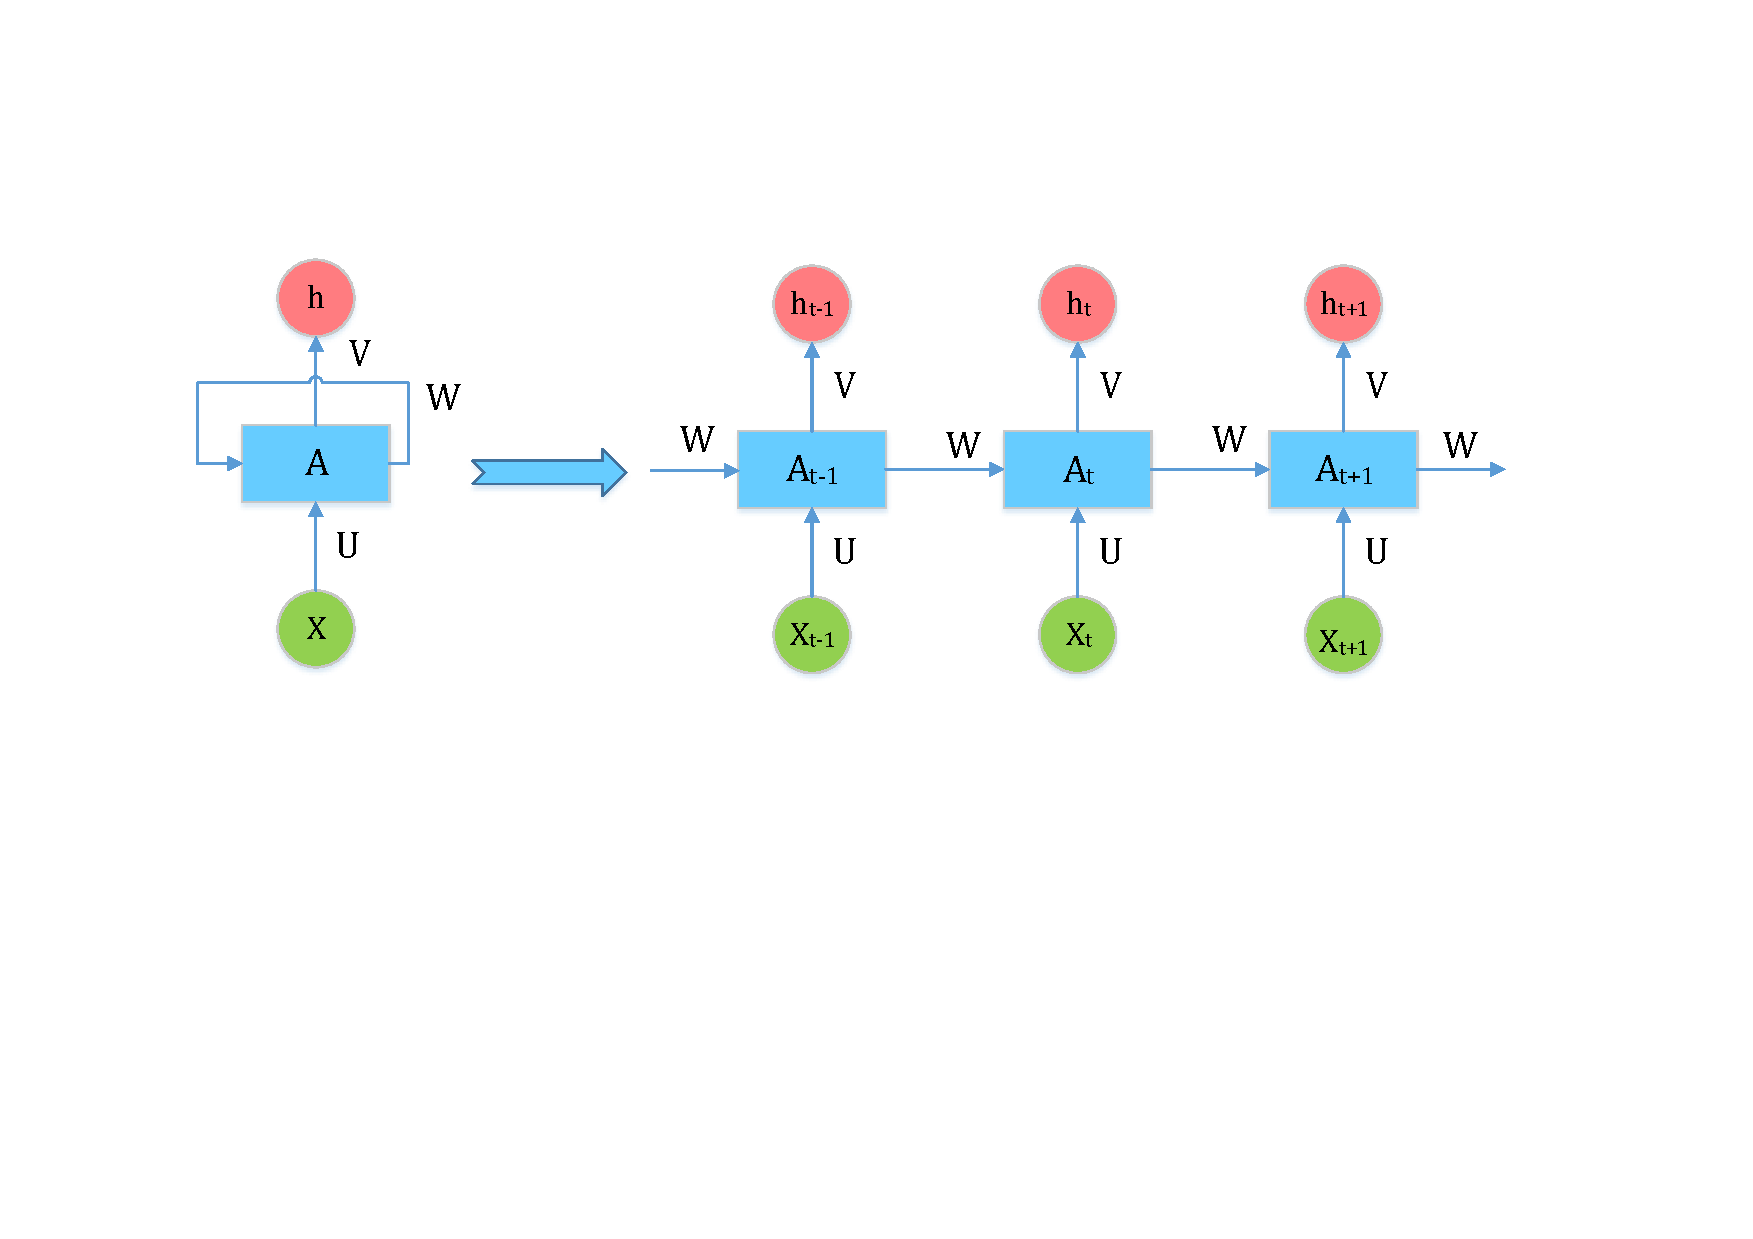
\includegraphics[scale=0.6]{figure/rnn.pdf}
\caption{Architecture of Recurrent Neural Network.}
\label{fig:rnn}
\end{figure}

In a traditional neural network, it is assumed that every input is independent of each other. While, in reality, sometimes, the processed information is in sequence. For example, in a sentence, the words may have relationship with other words. Much as Convolutional Neural Network is especially for data with grid of values, the Recurrent Neural Network is designed to make use of sequential information. The ``recurrent" refers to performing the same task for every element of a sequence, and the input of every node depends on previous computation.

The model of a classical RNN is shown in Figure~\ref{fig:rnn}. In the left of the graph, there is a computation node $\textbf{A}$, with an input $\textbf{X}$, an output for current node $\textbf{h}$. There is a weight $\textbf{W}$ which is utilized to compute next state. In this case, the computation of current state depends on previous computation results. The right side of the figure is the unfolding in time of the computation. From the figure, we can observe that
$$\textbf{A}_t = f(U\textbf{X}_t + W\textbf{A}_{t-1})$$
where $\textbf{A}_t$ is the hidden state of time $\textbf{t}$, $\textbf{X}_t$ is the input of current state, and function $\textbf{f}$ is the transition function for every time step. 

Though RNN is adapted to make use of sequential data, it is usually difficult to train the model. RNN maintains a vector of activations for each time step, which makes a RNN extremely deep~\cite{jozefowicz2015}. This also leads to the problem that it is difficult to learn long term dependencies with traditional RNN~\cite{bengio1994}. A recent summary by Pascanu et al.~\cite{pascanu2012} concluded the issues as the vanishing and the exploding gradient problems. There has been some work trying to solve the difficulty of training a RNN model. Hochreiter et al.~\cite{hochreiter1997} raised the Long Short-Term Memory (LSTM) architecture, which addresses the problem by re-parametrizing the RNN. Another model, Gated Recurrent Unit (GRU) was first presented by Cho et al.~\cite{cho2014}, is to make each unit to capture dependencies of different time scales. Chung et al.~\cite{chung2014} later evaluated LSTM and GRU on sequence modeling and found that GRU is comparable to LSTM. In our work, regarding RNN, we concentrate on LSTM.

The architecture of LSTM is shown in Figure~\ref{fig:lstm}. The first layer for LSTM is the ``forget gate layer". In this layer, the model checks $h_{t-1}$ and $x_t$, and outputs a value to represent how much information it needs to keep from previous states. 
$$f_t = \sigma (W_f \cdot [h_{t-1}, x_t] + b_f)$$
The second step consists the ``input gate layer" and a tanh layer. The ``input gate layer" is a sigmoid layer, which is used to decide what values the model needs to update. And the tanh layer creates a new vector, $\tilde{C}_t$, which could be added to current unit. 
\begin{align*}
i_t = \sigma (W_i \cdot [h_{t-1}, x_t] + b_i) \\
\tilde{C}_t = tanh(W_c \cdot [h_{t-1}, x_t] + b_C)
\end{align*}
And next, the model will obtain $C_t$ from multiplying old state by $f_i$, multiplying $\tilde{C}_t$ by $i_t$ and summing them up. 
$$C_t = f_t * C_{t-1} + i_t * \tilde{C}_t$$
Finally, the model needs to decide the output. The output gate layer implements operations on $C_t$ and $o_t$, and output $h_t$ for the next state.
\begin{align*}
o_t = \sigma (W_o [h_{t-1}, x_t] + b_o) \\
h_t = o_t * tanh(C_t)
\end{align*}

\begin{figure}
\centering
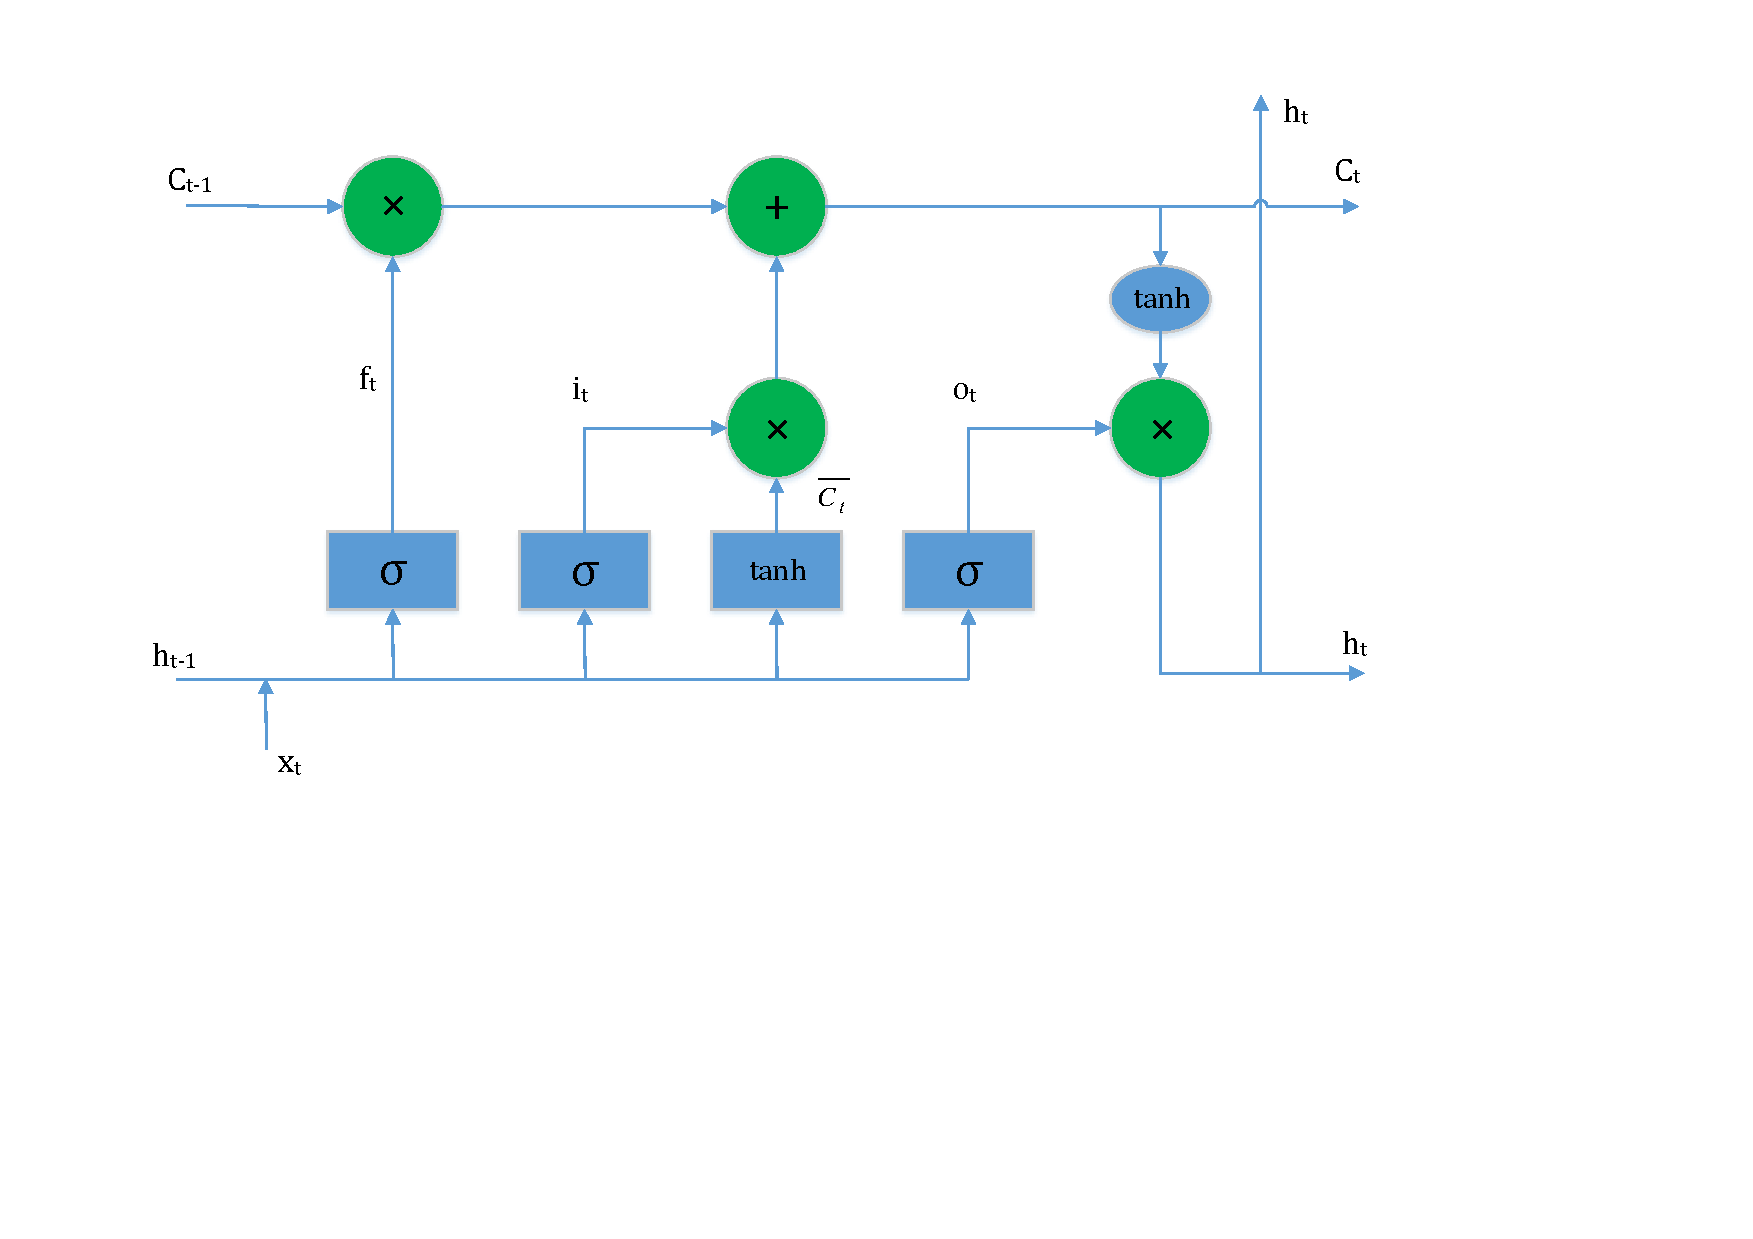
\includegraphics[scale=0.6]{figure/lstm.pdf}
\caption{Architecture of Long Short-Term Memory.}
\label{fig:lstm}
\end{figure}